\section{Introduction}\label{section:Intro}


%The Large Underground Xenon (LUX) experiment has reported results from a WIMP dark matter 
%search making use of its complete dataset. As reported in Ref.~\cite{Run4Paper}, no 
%evidence for WIMP scattering events is found, and restrictive bounds on the allowed dark 
%matter parameter space are derived.

%The LUX WIMP target material is 250 active kg of liquefied xenon (LXe) 
%instrumented as a dual phase time 
%projection chamber (TPC). Scintillation light from ionizing events, known
%as S1, is collected by arrays of photomultiplier tubes (PMTs) located above and below the liquid, 
%while liberated charge from the event is collected by an anode located several centimeters above the liquid
%surface. The anode region electric field is sufficient to generate secondary scintillation, known
%as S2, from the charge deposit, which is also measured and localized in the $xy$ plane by the 
%same PMT arrays. The $z$ coordinate of the event location is inferred
%from the drift time between the S1 and S2 signals. A complete description of the detector is given in Ref.~\cite{nimpaper}. 

%Background events in LUX typically result in electron recoil events, while the WIMPs are
%expected primarily create nuclear recoils. In LXe these event types can be statistically distinguished by 
%comparing the S1 and S2 signals of each event, since nuclear recoils create less
%S2 than electron recoils for the same S1. The LUX WIMP search fits the S1 and S2 signals
%of the WIMP search data to electron recoil and nuclear recoil models determined by tritium and neutron
%calibration data.

The LUX dark matter experiment makes extensive use of an $^{83m}$Kr 
calibration source dissolved into the bulk of the liquid xenon (LXe) fluid
to correct the detector response for spatial and time variations.
Ref.~\cite{scottspaper} describes how such efficiency corrections were 
derived and applied to the LUX 2013 WIMP search data (WS2013). 
Data collected by LUX between 2014 and 2016 (WS2014-16) is substantially 
more complex than that of WS2013 because the TPC suffered from a highly non-uniform and slowly time-varying 
drift field during this period. The WS2014-16 electric field is described in detail in Ref.~\cite{luciespaper},
where we report on a COMSOL model that accurately describes the field 
in three dimensions as a function of time. WIMP search results from the complete
LUX exposure are reported in Ref.~\cite{lux-complete}.

%
% are
%derived from such calibration data. In general
%the S1 signal depends on the event location due to the varying light collection efficiency, 
%while the S2 signal depends on $z$ due to charge attenuation and on $xy$ due to 
%anode gain variations. If the electric field is sufficiently uniform and constant, then any
%variation in the S1 and S2 signals, summed over 
%then the 32.1~keV and 9.4~keV decays, can be attributed to detector efficiency effects. The
%electric field condition is approximately satisfied by the LUX TPC in 2013, and appropriate 
%correction functions were derived from $^{83m}$Kr weekly calibration runs and applied to the 
%WS2013 search data.


%The model was developed by comparing the observed
%event locations in LUX $^{83m}$Kr calibration data to simulated drift trajectories from the model.

%The S1 and S2 yields in LXe depend on the electric field because of its effect on 
%the recombination probability. And owing to the non-uniform and time-varying electric field in WS2014-16, 
%the electron recoil band in this data, and, to a lesser extent, the nuclear recoil band, 
%depend on the event location and time. In the LUX WIMP search this complexity was managed
%by dividing the detector into four slices in $z$ and four time periods. 16 electron recoil bands and 
%16 nuclear recoil bands are determined for these detector conditions, and the data is compared
%to expectations in each of the 16 datasets. 

In this paper we report on the derivation and application of detector efficiency correction functions
that are tolerant to the non-uniform electric field. The 
correction functions so derived accurately characterize the light and charge collection efficiencies 
of the detector as a function of position and time, and are insensitive to the local electric field 
conditions. Such corrections are
appropriate to apply to all classes of single site events in LUX, 
including electron recoils and nuclear recoils, and spanning 
event energies of a few keV to hundreds of keV. 


%We note that field-insensitive corrections 
%are a requirement to properly interpret WIMP search data in the presence of a non-uniform field. 
%By definition, the recoil type of WIMP search data is not known on an event-by-event basis, 
%and so the detector corrections cannot contain any 



%We note
%that these corrections functions do not attempt to describe or correct 
%the genuine variation in the charge and light yields
%that result from the electric field non-uniformity. In fact, charge and light yield corrections 
%can not be made in WIMP search data even in principle, since these yields depend on the event type (electron
%recoil and nuclear recoil), which is unknown on an event-by-event basis.

The principle of operation of the LUX liquid xenon TPC is described in Ref.~\cite{lux-nim}. Briefly, 
we measure the scintillation (S1) and charge (S2) signals from ionizing events in the active 
liquid xenon
volume and extract all three position coordinates of each single-site event.
To derive detector efficiency correction functions from calibration data we make 
use of the same $^{83m}$Kr  calibration source that was described in Ref.~\cite{scottspaper}.
To neutralize the electric field effects that are present in the  $^{83m}$Kr calibration data, 
we artificially modify each dataset to appear as it would have if
the detector electric field had been uniform. We refer to this process as 'field-smoothing'. 
Remaining S1 and S2 variations in the calibration data can then be attributed to detector efficiency effects
alone, and corrections can be derived and applied to contemporaneous WIMP search data in the usual 
manner.\footnote{In the presence of a non-uniform field, efficiency correction 
functions naively derived without field-smoothing the $^{83m}$Kr data 
would not be applicable at other electron recoil energies, nor would they be applicable to nuclear
recoil events in WIMP search data.}
For the LUX WS2014-16 data, we choose to field-smooth the $^{83m}$Kr data to appear as it would in a 
uniform field of XXX V/cm. This is the value of the electric field at the center of
LUX in September 2015. 

The field-smoothing functions that we report reflect the fundamental charge and light
yield properties of the liquid xenon fluid, and they are applicable to any LXe TPC that makes
use of $^{83m}$Kr as a calibration source within the range of electric fields that we report.
Future dark matter searches such as LZ may benefit from these smoothing functions, 
even if the drift field of those experiments is less complex that the LUX Run 4 field. Indeed, 
all LXe TPCs experience some
field non-uniformities due to electrostatic effects such as wire grid transparency and charge
build-up, and in principle $^{83m}$Kr data from all such detectors may benefit from field smoothing.

The LUX detector is described in detail in Ref.~\cite{lux-nim}. We note here that ....




%We make use of a proxy observable
%that can be measured in each TPC volume element (voxel) and in each $^{83m}$Kr calibration dataset. 
%This observable, which we refer to as S1a/S1b, depends only on the local electric field of the voxel.

%has a one-to-one dependence on the local electric field in each three dimensional voxel
%of the detector. The observable is , the ratio of the S1 signal from the 32.1~keV and 9.4~keV
%$^{83m}$Kr decays. We derive data alteration functions that relate how the charge and light signals
%should be modified in each voxel in order to reproduce how the S1 and S2 signals would 
%have appeared had the field been XXX V/cm everywhere.


%are applicable to a



%As with all dual-phase TPCs, the S1 and S2 signals varied according to the vertex position of the interaction.  These signal variations resulted from both detector inefficiencies and field induced effects.  In the case of detector inefficiencies, the detection efficiency of S1 photons was roughly 30\% larger for events close to the cathode, when compared to those at the liquid surface. Similarly, loss of electrons to electronegativity impurities resulted in depth-dependent variation in the S2 signal, with 20-50\% of electrons liberated at the bottom of the detector reaching the liquid surface, depending on the purity of the liquid xenon at the time.  These sources of pulse area variations are independent of the energy of an event, or the type of recoil interaction that occurred, and can therefore be removed by applying event-agnostic position dependent signal corrections as was done in~\ref{Run3Reanalysis}.  Note that these energy and recoil-independent signal variations will be referred to as "detector inefficiencies" throughout this paper. 




%As detailed in~\ref{Run4Paper}, the anode, gate, and cathode grids underwent a conditioning campaign inbetween LUX's WS2013 and WS2014–16 data collections.  This campaign increased the operating extraction field from 2.9 kV/cm to 3.5 kV/cm, and the detector's electron extraction efficiency from 49$\pm$3\% to 73$\pm$4\%.  After completing the grid conditioning campaign, deviations in the trajectory of free electrons, as well as inconsistencies in electron lifetime measurements across multiple sources, led to the conclusion that a non-uniform and time-varying negative
%charge density in the polytetrafluoroethylene (PTFE)
%panels had developed during the campaign.


%%%%%%%%%%%%%%%%%%%%%%%%
% Old Fig 1: Nest yields for light and charge
%%%%%%%%%%%%%%%%%%%%%%%
%\begin{center}
%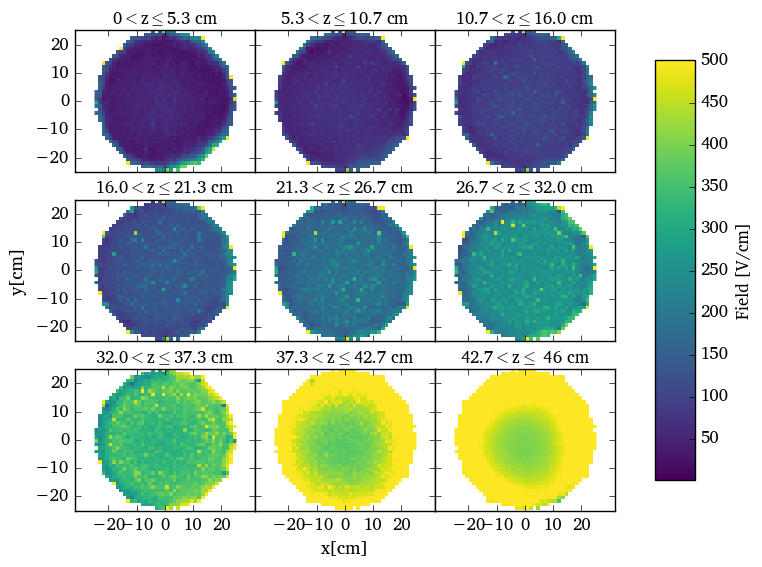
\includegraphics[scale=0.25]{figures/Fig1.png}
%\captionof{figure}{Predictions from NEST for the light yield (top row) and charge yield (bottom row) of electron recoil event from gamma ray interaction (left column) and beta particle interaction (right column).  Field values are indicated by the colored lines.  Light yield and charge yield have less dependence on the field strength for lower energy events.  \cite{RecombSource} }
%\label{fig:LYQY}
%\end{center}
